\documentclass{beamer}
\usetheme[faculty=med]{fibeamer}
\usepackage[utf8]{inputenc}
\usepackage[
  main=english
]{babel}        %% typeset as follows:
%% These macros specify information about the presentation
\title{Teoria da Computação} %% that will be typeset on the
\subtitle{Decidibilidade} %% title page.
\author{Guilherme Meira}
%% These additional packages are used within the document:
\usepackage{ragged2e}  % `\justifying` text
\usepackage{booktabs}  % Tables
\usepackage{tabularx}
\usepackage{tikz}      % Diagrams
\usetikzlibrary{calc, shapes, backgrounds, positioning, fit, automata}
\usepackage{minted}
\usepackage{amsmath, amssymb}
\usepackage{url}       % `\url`s
\usepackage{listings}  % Code listings
\usepackage{xcolor}
\usepackage{subcaption}
\usepackage{textcomp}
\usepackage{spot}
\usepackage{cancel}
\usepackage{amsmath}
\usepackage[scr]{rsfso}
\newcommand{\TuringInput}{a,b,c,d,0,1,0,0,2}
\newcommand{\TuringHead}{5}
\newcommand{\TuringHeadColor}{orange}
\newcommand{\TuringState} {$q_{1}$}
\newcommand{\TuringRightEnd} {$\ldots$}
\newcommand{\TuringLeftEnd} {$\ldots$}
\newcommand{\TuringMachine}{\begin{tikzpicture}[
	tape pos/.style={
		draw=blue!50,
		fill=blue!20,
		minimum size=6mm,
		text height=3mm,
		node distance=0
	},
	tape head/.style={
		draw=\TuringHeadColor,
		rounded corners,
		very thick,
		fit=(tape \TuringHead),
		inner sep=1mm
	},
	tape start/.style={
		minimum size=6mm,
		text height=3mm,
		node distance=0
	},
	tape end/.style={
		minimum size=6mm,
		text height=3mm,
		node distance=0
	},
	machine state/.style={
		draw=\TuringHeadColor,
		below=of tape head,
		minimum size=6mm,
		very thick
	}
]
	\node[tape start] (tape 0) at (0,0) {\TuringLeftEnd};
	\providecommand\lastP 0
	\foreach \l [count=\p from 1, remember=\p as \prevP (initially 0)] in \TuringInput {
		\node[tape pos, right=of tape \prevP] (tape \p) {\l};
		\global\let\lastP\p
	};
	\node[tape end, right=of tape \lastP] {\TuringRightEnd};
	\node[tape head] (tape head) {};
	\node[machine state] {\TuringState}
		edge[->,\TuringHeadColor, very thick] (tape head);
		
\end{tikzpicture}}
\definecolor{highlightcolor}{RGB}{255, 140, 119}
\setminted{highlightcolor=highlightcolor}
\frenchspacing
\begin{document}
  \frame{\maketitle}
  \AtBeginSection[]{% Print an outline at the beginning of sections
  	\begin{frame}<beamer>
  		\frametitle{Agenda}
  		\tableofcontents[currentsection]
  	\end{frame}}
  	
\section{Algoritmos}
\begin{frame}{Algoritmos}
	O que é um algoritmo?\pause
	\begin{itemize}
		\item Informalmente: é uma coleção de instruções simples para realizar alguma tarefa
		\begin{itemize}
			\item \textbf{Exemplo:} uma receita
		\end{itemize}
		\item Até o século XX não havia uma definição precisa do que é um algoritmo
	\end{itemize}
\end{frame}
\begin{frame}{Algoritmos}
	\framesubtitle{Problemas de Hilbert}
	\begin{itemize}
		\item Em 1900, o matemático David Hilbert apresentou 23 problemas matemáticos que seriam desafios para o novo século
	\end{itemize}
	\begin{figure}
		\includegraphics[width=0.3\paperwidth]{resources/hilbert}
	\end{figure}
\end{frame}
\begin{frame}{Algoritmos}
	\framesubtitle{Problemas de Hilbert}
	\begin{itemize}
		\item \textbf{Polinômios:}
		\begin{itemize}
			\item Um polinômio é uma soma de termos, onde cada termo é o produto de algumas variáveis e uma constante chamada de \textbf{coeficiente}
			\item \textbf{Exemplo:}
			\begin{equation*}
				6 \cdot x \cdot x \cdot x \cdot y \cdot z \cdot z = 6x^{3}yz^{2}
			\end{equation*}
			é um termo com coeficiente 6 e
			\begin{equation*}
				6x^{3}yz^{2} + 3xy^{2}-x^{3}-10
			\end{equation*}
			é um polinômio de 4 termos nas variáveis $x$, $y$ e $z$
			\item Vamos considerar apenas coeficientes inteiros
		\end{itemize}
	\end{itemize}
\end{frame}
\begin{frame}{Algoritmos}
	\framesubtitle{Problemas de Hilbert}
	\begin{itemize}
		\item \textbf{Polinômios:}
		\begin{itemize}
			\item A \textbf{raiz} de um polinômio é um conjunto de valores de suas variáveis que faz com que o valor do polinômio seja zero
			\item \textbf{Exemplo:} uma raiz de
			\begin{equation*}
			6x^{3}yz^{2} + 3xy^{2}-x^{3}-10
			\end{equation*}
			é $x = 5$, $y = 3$ e $z = 0$
			\item Essa raiz é \textbf{inteira} porque todas as variáveis recebem valores inteiros
			\item Alguns polinômios possuem raízes inteiras e outros não
		\end{itemize}
	\end{itemize}
\end{frame}
\begin{frame}{Algoritmos}
	\framesubtitle{Problemas de Hilbert}
	\begin{itemize}
		\item O décimo problema de Hilbert envolvia descrever um algoritmo que determinasse se um polinômio tem ou não uma raiz inteira
		\begin{itemize}
			\item Na época, ele não usou o termo ``algoritmo'', mas ``um processo de acordo com o qual possa ser determinado por um número finito de operações''
		\end{itemize}
		\item Hilbert aparentemente assumiu que o algoritmo deveria existir e que só precisava ser descoberto
		\item Hoje sabemos que não existe um algoritmo que resolva esse problema
		\item Chegar a essa conclusão exigiu a criação de uma definição precisa de um algoritmo
	\end{itemize}
\end{frame}
\begin{frame}{Algoritmos}
	\framesubtitle{A Tese de Church-Turing}
	\begin{itemize}
		\item Em 1936 foram publicados os artigos de Alonzo Church e Alan Turing, com suas definições de algoritmo
		\item Chuch propôs um sistema chamado Cálculo Lambda e Turing propôs as Máquinas de Turing
		\item Posteriormente, foi provado que as duas definições eram equivalentes
		\item A \textbf{Tese de Church-Turing} conecta a noção informal de algoritmos e a definição precisa por meio de Máquinas de Turing
	\end{itemize}
\end{frame}
\begin{frame}{Algoritmos}
	\framesubtitle{A Tese de Church-Turing}
	\begin{itemize}
		\item Vamos descrever o décimo problema de Hilbert na nossa terminologia. Seja:
		\begin{equation*}
			D = \{p\ |\ p\ \text{é um polinômio com raízes inteiras}\}
		\end{equation*}
		\item O décimo problema de Hilbert que saber se $D$ é decidível (não é)
		\item $D$ é Turing-reconhecível?
	\end{itemize}
\end{frame}
\begin{frame}{Algoritmos}
	\framesubtitle{A Tese de Church-Turing}
	\begin{itemize}
		\item Vamos considerar uma variante mais simples do problema: polinômios com somente uma variável, como $4x^{3} - 2x^{2} + x - 7$
		\begin{equation*}
			D_{1} = \{p\ |\ p \text{ é um polinômio em }x\text{ com uma raiz real}\}
		\end{equation*}
		\item A Máquina de Turing $M_{1}$ que reconhece $D_{1}$ é:
		
		$M_{1} = $``Para uma entrada $\langle p\rangle$ onde $p$ é um polinômio em $X$:
		\begin{enumerate}
			\item Calcule o valor de $p$ para os valores $0, 1, -1, 2, -2, 3, -3, \cdots$. Se em algum ponto, o valor do polinômio for zero, \textbf{aceite}''
		\end{enumerate}
	\end{itemize}
\end{frame}
\begin{frame}{Algoritmos}
	\framesubtitle{A Tese de Church-Turing}
	\begin{itemize}
		\item Se $p$ tem uma raiz inteira, $M_{1}$ eventualmente a encontrará e aceitará
		\item Se $p$ não tem uma raiz inteira, $M_{1}$ executará para sempre
		\item Para o caso de múltiplas variáveis, podemos utilizar uma máquina semelhante, que testa todas as combinações de variáveis
		\item Ambas as máquinas reconhecem, mas não decidem $D$
		\item No caso de $D_{1}$, podemos converter $M_{1}$ em um decisor porque é possível calcular os limites máximos até onde a raiz pode estar. Para o caso de múltiplas variáveis, é impossível
	\end{itemize}
\end{frame}
\begin{frame}{Algoritmos}
	\framesubtitle{Descrição de algoritmos}
	\begin{itemize}
		\item De agora para frente, vamos nos afastar das definições de baixo nível da Máquina de Turing e focarmos apenas nos algoritmos
		\item Descreveremos algoritmos em alto nivel, não nos preocupando com a fita ou a cabeça da Máquina de Turing
	\end{itemize}
\end{frame}
\begin{frame}{Algoritmos}
	\framesubtitle{Descrição de algoritmos}
	Considere a linguagem a seguir:
	
	\begin{equation*}
		A = \{\spot<2>{\langle} G \spot<2>{\rangle}\ |\ G\ \text{é um }\spot<3>{\text{grafo}}\ \spot<5>{\text{conectado}}\ \spot<4>{\text{não-direcionado}}\}
	\end{equation*}
	\only<2>{
		\begin{itemize}
			\item Utilizaremos esse símbolo para indicar \textbf{uma codificação de $G$}, isto é, uma forma de representar $G$ em uma string
			\item \textbf{Exemplo:} $\langle G \rangle = (1,2,3,4)((1,2),(2,3),(3,1),(1,4))$
		\end{itemize}
		\begin{figure}
			\includegraphics[width=0.2\paperwidth]{resources/graph}
		\end{figure}
	}
	\only<3>{
		\begin{itemize}
			\item Um \textbf{grafo} é uma estrutura composta de um conjunto de \textbf{nós} conectados por um conjunto de \textbf{arestas}
		\end{itemize}
	}
	
	\only<4>{
		\begin{itemize}
			\item O grafo é \textbf{não-direcionado} quando as arestas podem ser percorridas nos dois sentidos
		\end{itemize}
	}
	
	\only<5> {
		\begin{itemize}
			\item O grafo é \textbf{conectado} se é possível chegar a qualquer nó a partir de qualquer outro nó
		\end{itemize}
	}
\end{frame}
\begin{frame}{Algoritmos}
	\framesubtitle{Descrição de algoritmos}
	$M = $``Para uma entrada $\langle G\rangle$, que é a codificação de um grafo $G$:
	\begin{enumerate}
		\item Selecione o primeiro nó de $G$ e marque-o
		\item Repita até que nenhum novo nó seja marcado:
		\begin{itemize}
			\item Para cada nó de $G$, marque-o se existe uma aresta entre ele e um nó já marcado
		\end{itemize}
		\item Percorra todos os nós de $G$ para determinar se eles estão todos marcados. Se sim, aceite, caso contrário, rejeite''
	\end{enumerate}
\end{frame}
\begin{frame}{Algoritmos}
	\framesubtitle{Descrição de algoritmos}
	\begin{figure}
		\only<1>{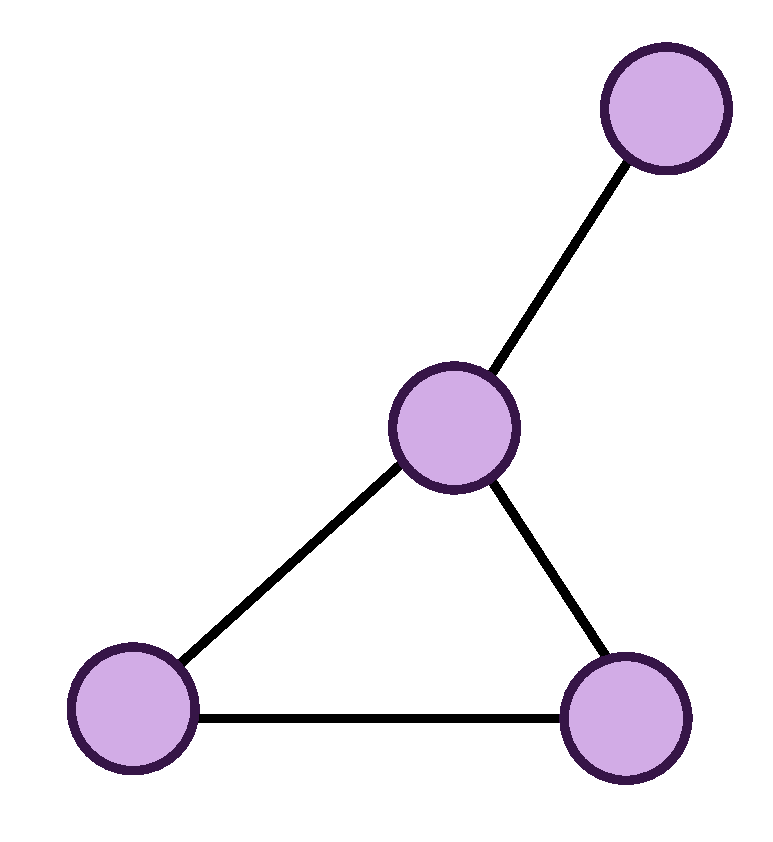
\includegraphics[width=0.4\paperwidth]{resources/grafo1}}
		\only<2>{\includegraphics[width=0.4\paperwidth]{resources/grafo2}}
		\only<3>{\includegraphics[width=0.4\paperwidth]{resources/grafo3}}
		\only<4>{\includegraphics[width=0.4\paperwidth]{resources/grafo4}}
		\only<5>{\includegraphics[width=0.4\paperwidth]{resources/grafo5}}
		\only<6>{\includegraphics[width=0.4\paperwidth]{resources/grafo6}}
		\only<7>{\includegraphics[width=0.4\paperwidth]{resources/grafo7}}
		\only<8>{\includegraphics[width=0.4\paperwidth]{resources/grafo8}}
		\only<9>{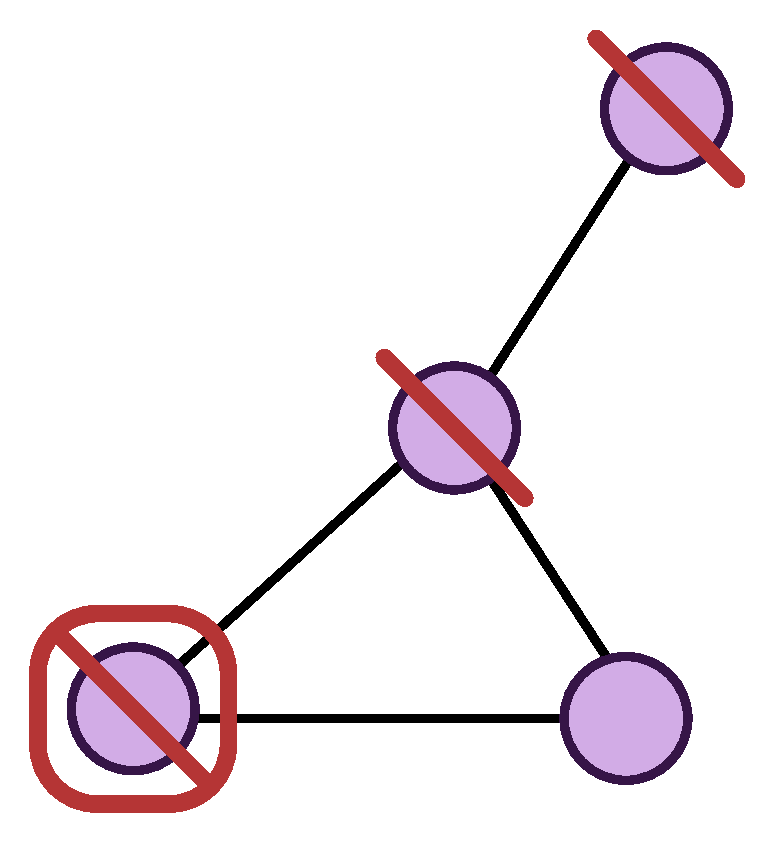
\includegraphics[width=0.4\paperwidth]{resources/grafo9}}
		\only<10>{\includegraphics[width=0.4\paperwidth]{resources/grafo10}}
		\only<11>{\includegraphics[width=0.4\paperwidth]{resources/grafo11}}
	\end{figure}
\end{frame}
\section{Indecidibilidade}
\begin{frame}{Indecidibilidade}
	\begin{itemize}
		\item Computadores são tão poderosos que parecem ser capazes de resolver qualquer problema
		\item Existem alguns problemas que não podem ser resolvidos
	\end{itemize}
\end{frame}
\begin{frame}{Indecidibilidade}
	Considere a linguagem:
	\begin{equation*}
		A_{TM} = \{\langle M,w\rangle\ |\ M\ \text{é uma Máquina de Turing e}\ M\ \text{aceita}\ w\}
	\end{equation*}\pause
	\begin{block}{Teorema}
		$A_{TM}$ é indecidível.
	\end{block}
\end{frame}
\begin{frame}{Indecidibilidade}
	Primeiramente, $A_{TM}$ é Turing-reconhecível?\pause
	
	$U = $``Para uma entrada $\langle M,w\rangle$, onde $M$ é uma Máquina de Turing e $w$ é uma string:
	\begin{enumerate}
		\item Simule $M$ com uma entrada $w$
		\item Se $M$ aceitar, aceite. Se $M$ rejeitar, rejeite''
	\end{enumerate}
	
	Se $M$ entrar em loop, $U$ também entra em loop (não é um decisor).
\end{frame}
\begin{frame}{Indecidibilidade}
	\framesubtitle{O método da diagonalização}
	\begin{itemize}
		\item Para provar a indecidibilidade de $A_{TM}$, utilizamos uma técnica chamada \textbf{diagonalização}
		\item Esse método foi descoberto por Georg Cantor, em 1873
	\end{itemize}
	\begin{figure}
		\includegraphics[width=0.3\paperwidth]{resources/cantor}
	\end{figure}
\end{frame}
\begin{frame}{Indecidibilidade}
	\framesubtitle{O método da diagonalização}
	\begin{itemize}
		\item Considere dois conjuntos, $A=\{1,3,5,7,9\}$ e $B=\{2,3,4\}$
		\item Qual dos dois é maior?\pause
		\item $A$ tem 5 elementos, enquanto $B$ tem apenas 3. $A$ é maior\pause
		\item E se $A$ e $B$ forem infinitos?
	\end{itemize}
\end{frame}
\begin{frame}{Indecidibilidade}
	\framesubtitle{O método da diagonalização}
	\begin{itemize}
		\item No caso de conjuntos infinitos, não podemos utilizar contagem
		\item Cantor considera que dois conjuntos tem o mesmo tamanho se pudermos \textbf{emparelhar todos os elementos de um conjunto nos elementos do outro}
	\end{itemize}
\end{frame}
\begin{frame}{Indecidibilidade}
	\framesubtitle{O método da diagonalização}
	Seja $\mathscr{N}$ o conjunto dos números naturais $\{1,2,3,\cdots\}$ e $\mathscr{E}$ o conjunto dos números naturais pares $\{2,4,6,\cdots\}$. Qual conjunto é maior?\pause
	
	A \textbf{correspondência} $f$ que mapeia $\mathscr{N}$ para $\mathscr{E}$ é $f(n) = 2n$.
	
	\begin{table}[!b]
		{\carlitoTLF
			\begin{tabular}{ccc}
				\textbf{n} & \textbf{f(n)} \\
				\toprule
				1 & 2 \\
				2 & 4 \\
				3 & 6 \\
				$\vdots$ & $\vdots$ \\
				\bottomrule
			\end{tabular}}
		\end{table}
\end{frame}
\begin{frame}{Indecidibilidade}
\framesubtitle{O método da diagonalização}
	\begin{block}{Definição}
		Um conjunto $A$ é \alert{contável} se ele for finito ou se tiver o mesmo tamanho que $\mathscr{N}$.
	\end{block}
\end{frame}
\begin{frame}{Indecidibilidade}
	\framesubtitle{O método da diagonalização}
	Considere o conjunto dos números racionais positivos:
	\begin{equation*}
		\mathscr{Q} = \left\{\frac{m}{n}\ |\ m,n \in \mathscr{N} \right\}
	\end{equation*}
	$\mathscr{Q}$ é maior que $\mathscr{N}$?
\end{frame}
\begin{frame}{Indecidibilidade}
	\framesubtitle{O método da diagonalização}
	\begin{figure}
		\only<1>{\includegraphics[width=0.4\paperwidth]{resources/cantor1}}
		\only<2>{\includegraphics[width=0.4\paperwidth]{resources/cantor2}}
	\end{figure}
\end{frame}
\begin{frame}{Indecidibilidade}
	\framesubtitle{O método da diagonalização}
	Considere, agora, o conjunto $\mathscr{R}$ dos números reais. São números reais:
	\begin{itemize}
		\item $\pi = 3.1415926...$
		\item $\sqrt{2} = 1.4142135...$
	\end{itemize}
	O conjunto dos reais é contável?
	\begin{block}{Teorema}
		$\mathscr{R}$ é incontável.
	\end{block}
\end{frame}
\begin{frame}{Indecidibilidade}
	\framesubtitle{O método da diagonalização}
	Vamos tentar mapear todos os reais para os naturais:
	\begin{table}[!b]
	{\carlitoTLF
		\begin{tabular}{cc}
			\textbf{n} & \textbf{f(n)} \\
			\toprule
			1 & 3.14159... \\
			2 & 55.55555... \\
			3 & 0.12345... \\
			4 & 0.50000... \\
			$\vdots$ & $\vdots$ \\
			\bottomrule
		\end{tabular}}
	\end{table}
	Todos os números reais estão listados aqui?
\end{frame}
\begin{frame}{Indecidibilidade}
	\framesubtitle{O método da diagonalização}
	\begin{table}[!b]
	{\carlitoTLF
		\begin{tabular}{cc}
				\textbf{n} & \textbf{f(n)} \\
				\toprule
				1 & 3.\textcolor{red}{\textbf{1}}4159... \\
				2 & 55.5\textcolor{red}{\textbf{5}}555... \\
				3 & 0.12\textcolor{red}{\textbf{3}}45... \\
				4 & 0.500\textcolor{red}{\textbf{0}}0... \\
				$\vdots$ & $\vdots$ \\
				\bottomrule
		\end{tabular}}
	\end{table}
	O número $x = 0.4641...$ não está na tabela.
\end{frame}
\begin{frame}{Indecidibilidade}
	\framesubtitle{O método da diagonalização}
	O conjunto de Máquinas de Turing é contável?\pause
	\begin{itemize}
		\item Toda Máquina de Turing pode ser representada por uma string $\langle M\rangle$
		\item Se representamos cada Máquina de Turing com uma string de um alfabeto $\Sigma$, podemos listar todas as strings utilizando esse alfabeto
		\item Começamos pelas strings de comprimento 0, depois 1, depois 2 e assim sucessivamente
	\end{itemize}
\end{frame}
\begin{frame}{Indecidibilidade}
	\framesubtitle{O método da diagonalização}
	\textbf{Exemplo:} suponha que $\Sigma=\{0,1\}$.
	\begin{table}[!b]
	{\carlitoTLF
		\begin{tabular}{cc}
			\textbf{n} & \textbf{f(n)} \\
			\toprule
			1 & $\epsilon$ \\
			2 & 0 \\
			3 & 1 \\
			4 & 00 \\
			5 & 01 \\
			6 & 10 \\
			7 & 11 \\
			8 & 100 \\
			$\vdots$ & $\vdots$ \\
			\bottomrule
		\end{tabular}}
	\end{table}
\end{frame}
\begin{frame}{Indecidibilidade}
	\framesubtitle{O método da diagonalização}
	Portanto, o conjunto das Máquinas de Turing é \textbf{contável}.
	
	E o conjunto das linguagens?
\end{frame}
\begin{frame}{Indecidibilidade}
	\framesubtitle{O método da diagonalização}
	Vamos começar olhado o conjunto $\mathscr{B}$ de todas as sequências binárias infinitas. $\mathscr{B}$ 
	é contável ou incontável?\pause
	\begin{table}[!b]
	{\carlitoTLF
		\begin{tabular}{cc}
			\textbf{n} & \textbf{f(n)} \\
			\toprule
			1 & \textcolor{red}{\textbf{1}}00101010... \\
			2 & 0\textcolor{red}{\textbf{1}}0110101... \\
			3 & 01\textcolor{red}{\textbf{0}}110001... \\
			4 & 100\textcolor{red}{\textbf{1}}01110... \\
			$\vdots$ & $\vdots$ \\
			\bottomrule
		\end{tabular}}
	\end{table}
	$x = 0010...$ não está na tabela. $\mathscr{B}$ é incontável.
\end{frame}
\begin{frame}{Indecidibilidade}
	\framesubtitle{O método da diagonalização}
	\begin{itemize}
		\item Considere um alfabeto $\Sigma$. O conjunto de todas as palavras formadas por esse alfabeto é $\Sigma^{*} = \{s_{1}, s_{2}, s_{3},\cdots\}$.
		\item Considere o conjunto $\mathscr{L}$ de todas as linguagens no alfabeto $\Sigma$
		\item Cada linguagem $A \in \mathscr{L}$ tem uma sequência equivalente em $\mathscr{B}$: o $i$-ésimo bit da sequência é 1 se $s_{i} \in A$  e 0 se $s_{i} \notin A$
	\end{itemize}
\end{frame}
\begin{frame}{Indecidibilidade}
	\framesubtitle{O método da diagonalização}
	\textbf{Exemplo:} $\Sigma=\{0,1\}$ e $A$ é a linguagem de todas as palavras que começam com zero
	\begin{equation*}
		\Sigma^{*} = \{\epsilon, 0, 1, 00, 01, 10, 11, 000, 001, \cdots\}
	\end{equation*}
	\begin{equation*}
		A = \{0, 00, 01, 000, 001, \cdots\}
	\end{equation*}
	\begin{equation*}
		\chi_{A} = 0 1 0 1 1 0 0 1 1 \cdots
	\end{equation*}\pause
	Podemos mapear cada elemento de $\mathscr{L}$ em um elemento de $\mathscr{B}$. Vimos que $\mathscr{B}$ 
	e incontável, logo, $\mathscr{L}$ também é \textbf{incontável}.
\end{frame}
\begin{frame}{Indecidibilidade}
	\framesubtitle{O método da diagonalização}
	O que sabemos até agora:
	\begin{itemize}
		\item O conjunto de todas as Máquinas de Turing é \textbf{contável}
		\item Uma Máquina de Turing reconhece uma única linguagem, logo, o conjunto das linguagens reconhecíveis é \textbf{contável}
		\item O conjunto de todas as linguagens é \textbf{incontável}
	\end{itemize}
	Logo...\pause
	\begin{block}{Corolário}
		Algumas linguagens não são Turing-reconhecíveis.
	\end{block}
\end{frame}
\begin{frame}{Indecidibilidade}
	\framesubtitle{Uma linguagem indecidível}
	Agora, podemos provar que a linguagem $A_{TM}$ é indecidível:
	\begin{equation*}
		A_{TM} = \{\langle M,w\rangle\ |\ M\ \text{é uma Máquina de Turing e}\ M\ \text{aceita}\ w\}
	\end{equation*}
\end{frame}
\begin{frame}{Indecidibilidade}
	\framesubtitle{Uma linguagem indecidível}
	Vamos utilizar uma \textbf{prova por contradição}. Supomos que algo existe, e mostramos que isso gera contradição.
	\begin{itemize}
		\item Suponha que $H$ é um decisor para $A_{TM}$
		\item Para uma entrada $\langle M, w\rangle$, onde $M$ é uma Máquina de Turing e $w$ é uma string, $H$ para e aceita se $M$ aceita $w$. Além disso, $H$ para e rejeita se $M$ não aceitar $w$ ($M$ rejeita ou entra em loop). Em outras palavras:
		\begin{equation*}
			H\left(\langle M,w\rangle\right) = \begin{cases}
			aceita\text{ se }M\text{ aceita} \\
			rejeita\text{ se }M\text{ não aceita}
			\end{cases}
		\end{equation*}
	\end{itemize}
\end{frame}
\begin{frame}{Indecidibilidade}
	\framesubtitle{Uma linguagem indecidível}
	\begin{itemize}
		\item Agora, construa uma Máquina de Turing $D$ que utilize $H$ como uma subrotina
		\item $D$ chama $H$ para determinar o que $M$ faz quando recebe como entrada sua própria descrição $\langle M\rangle$. Quando $D$ recebe uma resposta de $H$, ela faz o oposto, isto é, se $H$ aceita, $D$ rejeita e vice-versa
	\end{itemize}
	$D = $``Para uma entrada $\langle M\rangle$, onde $M$ é uma Máquina de Turing:
	\begin{enumerate}
		\item Rode $H$ na entrada $\langle M, \langle M\rangle\rangle$
		\item Se $H$ aceita, \textbf{rejeite}. Se $H$ rejeita, \textbf{aceite}''
	\end{enumerate}
\end{frame}
\begin{frame}{Indecidibilidade}
	\framesubtitle{Uma linguagem indecidível}
	Em outras palavras:
	\begin{equation*}
	D\left(\langle M\rangle\right) = \begin{cases}
	aceita\text{ se }M\text{ não aceita }\langle M\rangle \\
	rejeita\text{ se }M\text{ aceita }\langle M\rangle
	\end{cases}
	\end{equation*}
	O que acontece quando passamos a descrição $\langle D\rangle$ como entrada para $D$?
\end{frame}
\begin{frame}{Indecidibilidade}
	\framesubtitle{Uma linguagem indecidível}
	\begin{figure}
		\includegraphics[width=0.8\paperwidth]{resources/halt}
	\end{figure}\pause
	Contradição! Portanto, $H$ e $D$ não podem existir.\pause
	
	https://www.youtube.com/watch?v=92WHN-pAFCs
\end{frame}
\begin{frame}{Indecidibilidade}
	\framesubtitle{Uma linguagem indecidível}
	Onde entra a diagonalização nessa prova?\pause
	
	Vamos listar todas as Máquinas de Turing e todas as descrições dessas máquinas. Na tabela abaixo, vemos o resultado de passar a descrição de uma máquina como parâmetro para outra:
	
	\begin{table}[!b]
		{\carlitoTLF
			\begin{tabular}{c|ccccc}
				& \textbf{$\langle M_{1}\rangle$} & \textbf{$\langle M_{2}\rangle$} & \textbf{$\langle M_{3}\rangle$} & \textbf{$\langle M_{4}\rangle$} & $\cdots$ \\
				\hline
				$M_{1}$ & $aceita$ & & $aceita$ & & \\
				$M_{2}$ & $aceita$ & $aceita$ & $aceita$ & $aceita$ & \\
				$M_{3}$ & & & & & \\
				$M_{4}$ & $aceita$ & $aceita$ & & & \\
				$\vdots$ & $\vdots$ & $\vdots$ & $\vdots$ & $\vdots$ & \\
			\end{tabular}}
		\end{table}
\end{frame}
\begin{frame}{Indecidibilidade}
	\framesubtitle{Uma linguagem indecidível}
	O resultado de rodar $H$ com as entradas da tabela anterior são representados abaixo:
	
\begin{table}[!b]
	{\carlitoTLF
		\begin{tabular}{c|ccccc}
			& \textbf{$\langle M_{1}\rangle$} & \textbf{$\langle M_{2}\rangle$} & \textbf{$\langle M_{3}\rangle$} & \textbf{$\langle M_{4}\rangle$} & $\cdots$ \\
			\hline
			$M_{1}$ & $aceita$ & $rejeita$ & $aceita$ & $rejeita$ & \\
			$M_{2}$ & $aceita$ & $aceita$ & $aceita$ & $aceita$ & \\
			$M_{3}$ & $rejeita$ & $rejeita$ & $rejeita$ & $rejeita$ & \\
			$M_{4}$ & $aceita$ & $aceita$ & $rejeita$ & $rejeita$ & \\
			$\vdots$ & $\vdots$ & $\vdots$ & $\vdots$ & $\vdots$ & \\
		\end{tabular}}
	\end{table}
\end{frame}
\begin{frame}{Indecidibilidade}
	\framesubtitle{Uma linguagem indecidível}
	Como $D$ é uma Máquina de Turing, ela deve aparecer nessa tabela
	
	\begin{table}[!b]
	{\carlitoTLF
		\begin{tabular}{c|ccccccc}
			& \textbf{$\langle M_{1}\rangle$} & \textbf{$\langle M_{2}\rangle$} & \textbf{$\langle M_{3}\rangle$} & \textbf{$\langle M_{4}\rangle$} & $\cdots$ & \textbf{$\langle D\rangle$} & $\cdots$ \\
			\hline
			$M_{1}$ & \underline{$aceita$} & $rejeita$ & $aceita$ & $rejeita$ & $\cdots$ & $aceita$ & \\
			$M_{2}$ & $aceita$ & \underline{$aceita$} & $aceita$ & $aceita$ & $\cdots$ & $aceita$ & \\
			$M_{3}$ & $rejeita$ & $rejeita$ & \underline{$rejeita$} & $rejeita$ & $\cdots$ & $rejeita$ & \\
			$M_{4}$ & $aceita$ & $aceita$ & $rejeita$ & \underline{$rejeita$} & $\cdots$ & $aceita$ & \\
			$\vdots$ & $\vdots$ & $\vdots$ & $\vdots$ & $\vdots$ & & & \\
			$D$ & $rejeita$ & $rejeita$ & $aceita$ & $aceita$ & $\cdots$ & ? & \\
		\end{tabular}}
	\end{table}
	A contradição ocorre no ``?'', onde a saída da máquina deve ser o oposto dela mesma.
\end{frame}
\begin{frame}{Indecidibilidade}
	\framesubtitle{Uma linguagem irreconhecível}
	Até agora, vimos que existem linguagens que não podem ser decididas (como $A_{TM}$). Existem linguagens que sequer podem ser reconhecidas. Antes de vermos uma dessas linguagens, precisamos conhecer alguns conceitos novos:
	\begin{itemize}
		\item O \textbf{complemento} de uma linguagem é a linguagem formada por todas as palavras que \textbf{não} pertencem a uma linguagem
		\item Uma linguagem é \textbf{co-Turing-reconhecível} se o seu complemento é Turing-reconhecível
	\end{itemize}\pause
	\begin{block}{Teorema}
		Uma linguagem é decidível se, e somente se ela é Turing-reconhecível e co-Turing-reconhecível.
	\end{block}
\end{frame}
\begin{frame}{Indecidibilidade}
	\framesubtitle{Uma linguagem irreconhecível}
	Precisamos provar duas direções desse teorema.
	\begin{itemize}
		\item \textbf{1)} Se $A$ é decidível, então $A$ e $\overline{A}$ são Turing-reconhecíveis
	\end{itemize}
	Toda linguagem decidível é Turing-reconhecível, e o complemento de uma linguagem decidível também é decidível.
\end{frame}
\begin{frame}{Indecidibilidade}
	\framesubtitle{Uma linguagem irreconhecível}
	\begin{itemize}
		\item \textbf{2)} Se $A$ e $\overline{A}$ são Turing-reconhecíveis, então $A$ é decidível
	\end{itemize}
	Seja $M_{1}$ um reconhecedor de $A$ e $M_{2}$ um reconhecedor de $\overline{A}$. A Máquina de Turing a seguir é um decisor de $A$:
	$M = $``Para uma entrada $w$:
	\begin{enumerate}
		\item Execute as máquinas $M{1}$ e $M_{2}$ em paralelo com a entrada $w$
		\item Se $M_{1}$ aceitar, \textbf{aceite}. Se $M_{2}$ aceitar, \textbf{rejeite}''
	\end{enumerate}
\end{frame}
\begin{frame}{Indecidibilidade}
	\framesubtitle{Uma linguagem irreconhecível}
	\begin{block}{Corolário}
		$\overline{A_{TM}}$ não é Turing-reconhecível.
	\end{block}
	
	Sabemos que $A_{TM}$ é Turing-reconhecível. Se $\overline{A_{TM}}$ também fosse Turing-reconhecível, $A_{TM}$ seria decidível. Sabemos que $A_{TM}$ não é decidível, portanto, $\overline{A_{TM}}$ não pode ser Turing-reconhecível.
\end{frame}
\end{document}